\begin{frame}\frametitle{Background Overview}

\centering
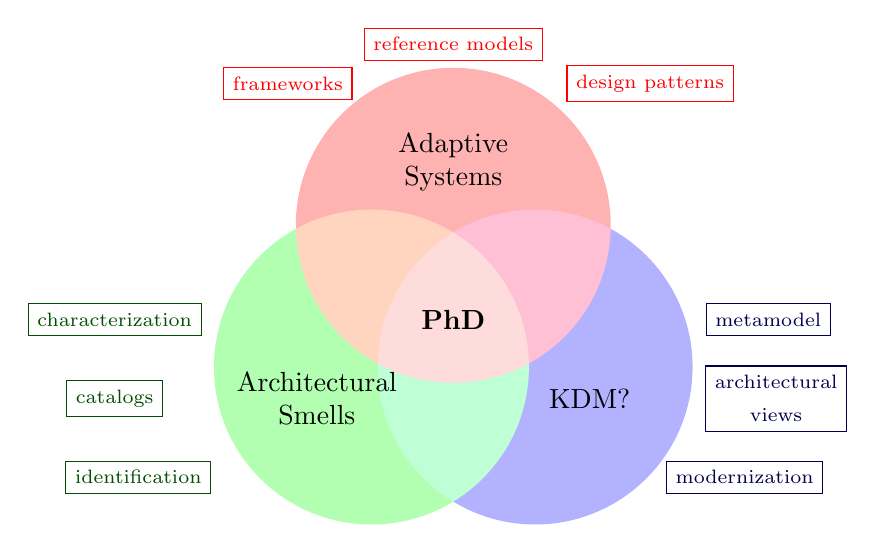
\begin{tikzpicture}
\onslide<1-> {

\begin{scope}[blend group = soft light]
\fill[red!30!white]   ( 90:1.2) circle (2);
\fill[green!30!white] (210:1.2) circle (2);
\fill[blue!30!white]  (330:1.2) circle (2);
\end{scope}


\node[align = center] at ( 90:2)    {Adaptive \\ Systems};
\node[align = center] at ( 210:2)   {Architectural \\ Smells};
\node[align = center] at ( 330:2)   {KDM?};
\node  {\textbf{PhD}};

}

\onslide<2-> {

\node[align = center, draw, rectangle, color= red] at ( -2.1,3)    {{\scriptsize frameworks}};
\node[align = center, draw, rectangle, color= red] at ( 0,3.5)    {{\scriptsize reference models}};
\node[align = center, draw, rectangle, color= red] at ( 2.5,3)    {{\scriptsize design patterns}};
}

\onslide<3-> {

\node[align = center, draw, rectangle, color= green!30!black] at (-4.3,0) {{\scriptsize characterization}}; 

\node[align = center, draw, rectangle, color= green!30!black] at (-4.3,-1) {{\scriptsize catalogs}};

\node[align = center, draw, rectangle, color= green!30!black] at (-4.0,-2) {{\scriptsize identification}};
}

\onslide<4->{

\node[align = center, draw, rectangle, color= blue!30!black] at (4.0,0) {{\scriptsize metamodel}};

\node[align = center, draw, rectangle, color= blue!30!black] at (4.1,-1) {{\scriptsize architectural} \\ {\scriptsize views}};

\node[align = center, draw, rectangle, color= blue!30!black] at (3.7,-2) {{\scriptsize modernization}};

}

\end{tikzpicture} 

\end{frame}
